\section{绘制阀盖主视图}
\begin{procedure}
\item 设置图层

建立“中心线”和“实线”两个图层,并将当前图层设置为“中心线”图层。
\item 绘制中心线

用xline命令绘制两条件相互垂直的构造线作为对称中心线。
\begin{lstlisting}
|命令: XLINE|
|指定点或 [水平(H)/垂直(V)/角度(A)/二等分(B)/偏移(O)]:25,25|
|指定通过点:$ @1<0$|
|指定通过点:$ @1<90$|
|指定通过点:|
\end{lstlisting}
绘制$\phi 39$中心线圆,其结果如图\ref{fig:fagaicenterline}所示。
\begin{lstlisting}
|命令: CIRCLE|
|指定圆的圆心或 [三点(3P)/两点(2P)/切点、切点、半径(T)]: 25,25|
|指定圆的半径或 [直径(D)]: 19.5|
\end{lstlisting}
\begin{figure}[htbp]
\centering
\subfloat[]{\label{fig:fagaicenterline}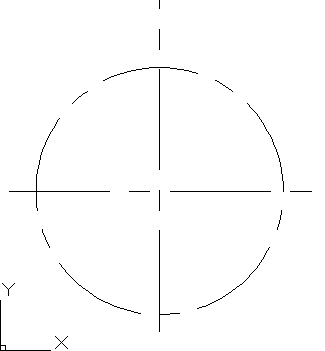
\includegraphics[scale=0.4]{fagaicenterline.png}}\hspace{30pt}
\subfloat[]{\label{fig:fagai1}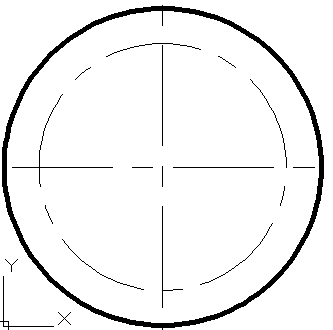
\includegraphics[scale=0.4]{fagai1.png}}\\
\subfloat[]{\label{fig:fagai2}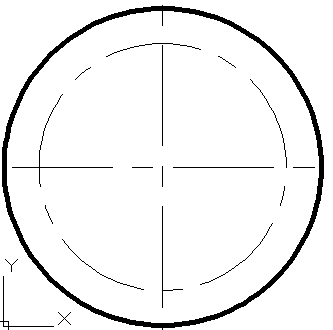
\includegraphics[scale=0.4]{fagai2.png}}\hspace{30pt}
\subfloat[]{\label{fig:fagai3}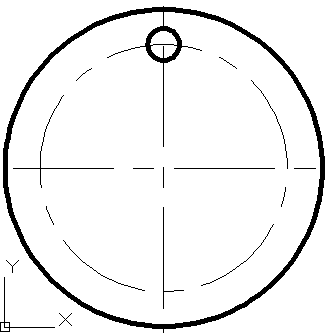
\includegraphics[scale=0.4]{fagai3.png}}
\caption{阀盖底板绘制过程}
\end{figure}
\item 绘制阀盖底板

将图层切换为实线层,并绘制$\phi 50$圆,其结果如图\ref{fig:fagai1} 所示。
\begin{lstlisting}
|命令: CIRCLE|
|指定圆的圆心或 [三点(3P)/两点(2P)/切点、切点、半径(T)]: 25,25|
|指定圆的半径或 [直径(D)]:$<$19.5000$>$ 25|
\end{lstlisting}
绘制$\phi 5$圆,其结果如图\ref{fig:fagai2}所示。
\begin{lstlisting}
|命令: CIRCLE|
|指定圆的圆心或 [三点(3P)/两点(2P)/切点、切点、半径(T)]: int 于|
|指定圆的半径或 [直径(D)]:$<$25.0000$>$ 2.5|
\end{lstlisting}
绘制$\phi 22$圓,其结果如图\ref{fig:fagai3}所示。
\begin{lstlisting}
|命令: CIRCLE|
|指定圆的圆心或 [三点(3P)/两点(2P)/切点、切点、半径(T)]: int 于|
|指定圆的半径或 [直径(D)]:$<$2.5000$>$ 11|
\end{lstlisting}
\item 绘制定位块

绘制$R21$圆弧。

启动圆弧命令的方法有:
\begin{itemize}
\item 键盘输入ARC\index{arc}或A。
\item 【绘图】$\rightarrow$【圆弧】项中的对应绘图子项。
\item 【绘图】$\triangleright$【圆弧】图标
\includegraphics[scale=0.6]{arc.png}.
\end{itemize}
采用第种方法或第三种方法启动命令后要求指写圆弧的起点。由于此图知道圆弧的中心点,故输入圆心选项字母,并用鼠标指定圆心。
\begin{figure}[htbp]
\centering
\subfloat[]{\label{fig:fagai4}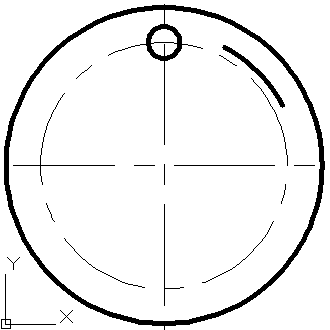
\includegraphics[scale=0.4]{fagai4.png}}\hspace{30pt}
\subfloat[]{\label{fig:fagai5}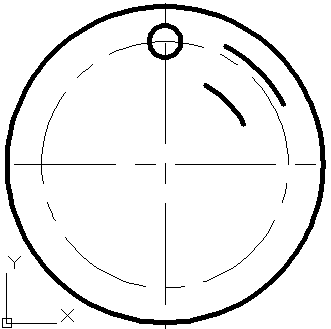
\includegraphics[scale=0.4]{fagai5.png}}\hspace{30pt}
\subfloat[]{\label{fig:fagai6}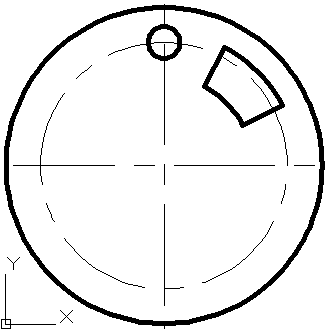
\includegraphics[scale=0.4]{fagai6.png}}
\caption{阀盖定位块绘制过程}
\end{figure}
\begin{lstlisting}
|命令: ARC|
|指定圆弧的起点或 [圆心(C)]: c 
|指定圆弧的圆心: int 于|
\end{lstlisting}
接下来指定圆弧的起点,默认情况下圆弧的绘图方向是逆时针方向,故需要从角度较小的点开始绘制。
\begin{lstlisting}
|指定圆弧的起点: $@21<27$|
\end{lstlisting}
指定圆弧角度,亦可指定另一个端点,其结果如图\ref{fig:fagai4}所示。
\begin{lstlisting}
|指定圆弧的端点或 [角度(A)/弦长(L)]:a|
|指定包含角: 36|
\end{lstlisting}
绘制$R14$圆弧,此处采用圆心、起点、端点法,其结果如图\ref{fig:fagai5}所示。
\begin{lstlisting}
|命令: ARC|
|指定圆弧的起点或 [圆心(C)]: c |
|指定圆弧的圆心: int 于|
|指定圆弧的起点: $@14<27$|
|指定圆弧的端点或 [角度(A)/弦长(L)]:$@14<63$|
\end{lstlisting}
绘制直线连接两圆弧端点,其结果如图\ref{fig:fagai6}所示。

\begin{lstlisting}
|命令: line|
|指定第一个点: end 于|
|指定下一点或 [放弃(U)]: end 于|
|指定下一点或 [放弃(U)]:|
|命令: line|
|指定第一个点: end 于|
|指定下一点或 [放弃(U)]: end 于|
|指定下一点或 [放弃(U)]:|
\end{lstlisting}
\item 阵列图形

阵列列$\phi 5$圆,其结果如图\ref{fig:fagai7}所示。
\begin{figure}[htbp]
\centering
\subfloat[]{\label{fig:fagai7}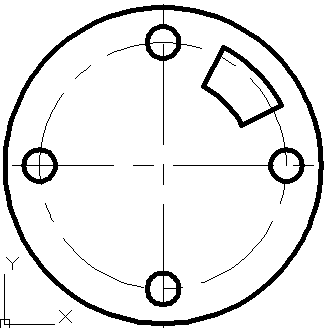
\includegraphics[scale=0.55]{fagai7.png}}\hspace{30pt}
\subfloat[]{\label{fig:fagai8}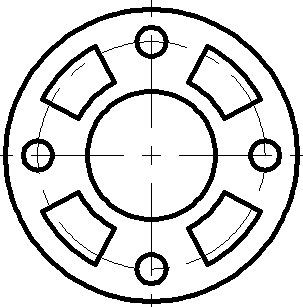
\includegraphics[scale=0.55]{fagai8.png}}
\caption{阀盖主视图阵列过程}
\end{figure}
\begin{lstlisting}
|命令: arraypolar|
|选择对象: 找到 1 个|
|选择对象:|
|类型 = 极轴  关联 = 否|
|指定阵列的中心点或 [基点(B)/旋转轴(A)]: int 于|
|选择夹点以编辑阵列或 [关联(AS)/基点(B)/项目(I)/项目间角度(A)/填|
|充角度(F)/行(ROW)/层(L)/旋转项目(ROT)/退出(X)] $<$退出$>$: i|
|输入阵列中的项目数或 [表达式(E)] $<$6$>$: 4|
|选择夹点以编辑阵列或 [关联(AS)/基点(B)/项目(I)/项目间角度(A)/填|
|充角度(F)/行(ROW)/层(L)/旋转项目(ROT)/退出(X)] $<$退出$>$:|
\end{lstlisting}

面域阀盖定位块。
\begin{lstlisting}
|命令: region|
|选择对象: 指定对角点: 找到 4 个|
|选择对象:|
|已提取 1 个环。|
|已创建 1 个面域。|
\end{lstlisting}
阵列阀盖定位块其结果如图\ref{fig:fagai8}所示。
\begin{lstlisting}
|命令: arraypolar|
|选择对象: 找到 1 个|
|选择对象:|
|类型 = 极轴  关联 = 否|
|指定阵列的中心点或 [基点(B)/旋转轴(A)]: int 于|
|选择夹点以编辑阵列或 [关联(AS)/基点(B)/项目(I)/项目间角度(A)/填|
|充角度(F)/行(ROW)/层(L)/旋转项目(ROT)/退出(X)] $<$退出$>$: i|
|输入阵列中的项目数或 [表达式(E)] $<$6$>$: 4|
|选择夹点以编辑阵列或 [关联(AS)/基点(B)/项目(I)/项目间角度(A)/填|
|充角度(F)/行(ROW)/层(L)/旋转项目(ROT)/退出(X)] $<$退出$>$:|
\end{lstlisting}
\end{procedure}
\endinput